\documentclass[12pt,notitlepage]{article}
\pagestyle{empty}
\usepackage[lmargin=0.4in,rmargin=0.4in,tmargin=.7in,bmargin=.7in]{geometry}                % See geometry.pdf to learn the layout options. There are lots.
\geometry{letterpaper}                   % ... or a4paper or a5paper or ... 
%\geometry{landscape}                % Activate for for rotated page geometry
%\usepackage[parfill]{parskip}    % Activate to begin paragraphs with an empty line rather than an indent
\usepackage{parskip}
\usepackage{graphicx}
%\usepackage{amssymb}
%\usepackage{epstopdf}
%%
%\usepackage{rotating}
%\usepackage{tikz}
%\usetikzlibrary{shapes,arrows}
%\usepackage{graphicx}
%\usepackage{tikz-dependency}
\usepackage{natbib}
\usepackage{url}
\usepackage{color,soul}
\usepackage{multirow}
\usepackage{fancyhdr}

%\DeclareGraphicsRule{.tif}{png}{.png}{`convert #1 `dirname #1`/`basename #1 .tif`.png}
\setlength{\parindent}{15pt} %Paragraphs will not be indented
%\parskip=10pt
\linespread{1.2}

%\title{PDT items}
%\author{Levi King \\ Last updated:}
\date{}

%\pagestyle{fancy}
%\fancyhf{}
%\fancyhead[C]{\textbf{PDT Items}}
%\renewcommand{\headrulewidth}{0pt}
%\fancyhead[RE,LO]{Guides and tutorials}
%\fancyfoot[CE,CO]{\leftmark}
%\fancyfoot[LE,RO]{\thepage}
\begin{document}
%\maketitle
All PDT items, 1-30:
\begin{center}
\begin{tabular}{|c||c||c||c||c|}
\hline
I01-IN & I02-TR & I03-DI & I04-IN & I05-DI \\

\includegraphics[width=0.13\columnwidth]{square/I01.jpg} & 
\includegraphics[width=0.13\columnwidth]{figures/I02.jpg} &  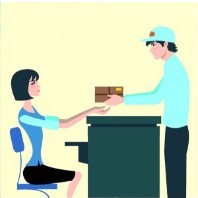
\includegraphics[width=0.13\columnwidth]{square/I03.jpg} &  
\includegraphics[width=0.13\columnwidth]{square/I04.jpg} & 
\includegraphics[width=0.13\columnwidth]{square/I05.jpg} \\
\hline
\hline
I06-TR & I07-IN & I08-DI & I09-TR & I10-IN \\

\includegraphics[width=0.13\columnwidth]{square/I06.jpg} &  
\includegraphics[width=0.13\columnwidth]{square/I07.jpg} &  
\includegraphics[width=0.13\columnwidth]{square/I08.jpg} & 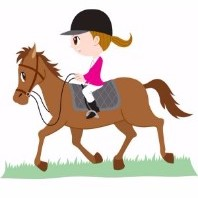
\includegraphics[width=0.13\columnwidth]{square/I09.jpg} & 
\includegraphics[width=0.13\columnwidth]{square/I10.jpg} \\
\hline
\hline
I11-DI & I12-TR & I13-IN & I14-DI & I15-TR \\

\includegraphics[width=0.13\columnwidth]{square/I11.jpg} &  
\includegraphics[width=0.13\columnwidth]{square/I12.jpg} & 
\includegraphics[width=0.13\columnwidth]{square/I13.jpg} & 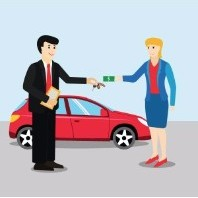
\includegraphics[width=0.13\columnwidth]{square/I14.jpg} &  
\includegraphics[width=0.13\columnwidth]{square/I15.jpg} \\
\hline
\hline
I16-TR & I17-DI & I18-IN & I19-TR & I20-IN \\

\includegraphics[width=0.13\columnwidth]{square/I16.jpg} & 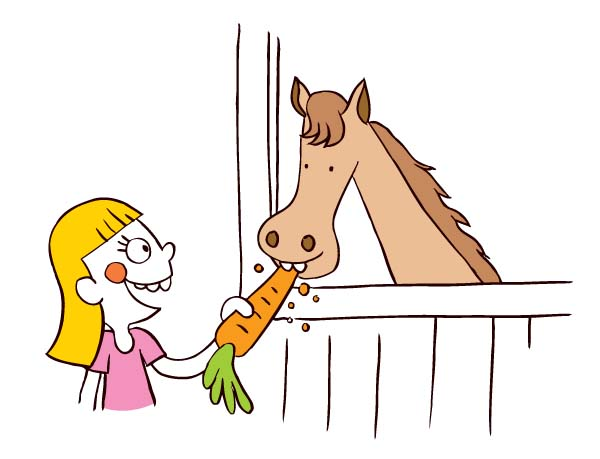
\includegraphics[width=0.13\columnwidth]{figures/I17.jpg} &  
\includegraphics[width=0.13\columnwidth]{square/I18.jpg} &  
\includegraphics[width=0.13\columnwidth]{square/I19.jpg} & 
\includegraphics[width=0.13\columnwidth]{square/I20.jpg} \\
\hline
\hline
I21-DI & I22-TR & I23-DI & I24-IN & I25-TR \\
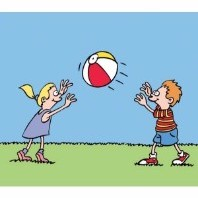
\includegraphics[width=0.13\columnwidth]{square/I21.jpg} &  
\includegraphics[width=0.13\columnwidth]{square/I22.jpg} &  
\includegraphics[width=0.13\columnwidth]{square/I23.jpg} & 
\includegraphics[width=0.13\columnwidth]{square/I24.jpg} & 
\includegraphics[width=0.13\columnwidth]{square/I25.jpg} \\
\hline
\hline
I26-DI & I27-IN & I28-DI & I29-TR & I30-IN \\

\includegraphics[width=0.13\columnwidth]{square/I26.jpg} &  
\includegraphics[width=0.13\columnwidth]{square/I27.jpg} & 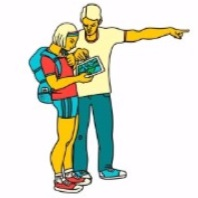
\includegraphics[width=0.13\columnwidth]{square/I28.jpg} & 
\includegraphics[width=0.13\columnwidth]{square/I29.jpg} &  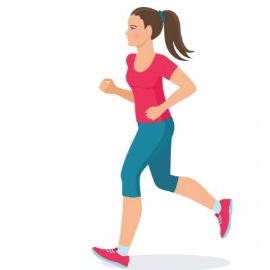
\includegraphics[width=0.13\columnwidth]{square/I30.jpg} \\
\hline
\end{tabular}
\vspace{1em} \\
\end{center}

\newpage

\begin{center}
\textbf{Intransitives:}

\begin{tabular}{|c||c||c||c||c|}

\hline

I01-IN & I04-IN & I07-IN & I010-IN & I13-IN \\

\includegraphics[width=0.13\columnwidth]{square/I01.jpg} & 
\includegraphics[width=0.13\columnwidth]{figures/I04.jpg} &  
\includegraphics[width=0.13\columnwidth]{square/I07.jpg} &  
\includegraphics[width=0.13\columnwidth]{square/I10.jpg} & 
\includegraphics[width=0.13\columnwidth]{square/I13.jpg} \\
\hline
\hline
I18-IN & I20-IN & I24-IN & I27-IN & I30-IN \\

\includegraphics[width=0.13\columnwidth]{square/I18.jpg} &  
\includegraphics[width=0.13\columnwidth]{square/I20.jpg} &  
\includegraphics[width=0.13\columnwidth]{square/I24.jpg} & 
\includegraphics[width=0.13\columnwidth]{square/I27.jpg} & 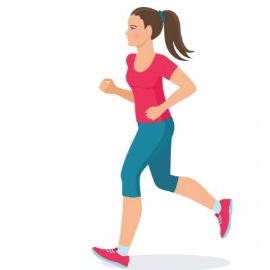
\includegraphics[width=0.13\columnwidth]{square/I30.jpg} \\
\hline
\end{tabular}

\textbf{Transitives:}

\begin{tabular}{|c||c||c||c||c|}
\hline
I02-TR & I06-TR & I09-TR & I12-TR & I15-TR \\

\includegraphics[width=0.13\columnwidth]{square/I02.jpg} &  
\includegraphics[width=0.13\columnwidth]{square/I06.jpg} & 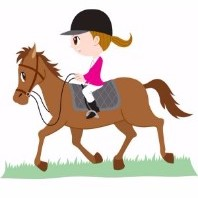
\includegraphics[width=0.13\columnwidth]{square/I09.jpg} & 
\includegraphics[width=0.13\columnwidth]{square/I12.jpg} &  
\includegraphics[width=0.13\columnwidth]{square/I15.jpg} \\
\hline
\hline
I16-TR & I19-TR & I22-TR & I25-TR & I29-TR \\

\includegraphics[width=0.13\columnwidth]{square/I16.jpg} & 
\includegraphics[width=0.13\columnwidth]{figures/I19.jpg} &  
\includegraphics[width=0.13\columnwidth]{square/I22.jpg} &  
\includegraphics[width=0.13\columnwidth]{square/I25.jpg} & 
\includegraphics[width=0.13\columnwidth]{square/I29.jpg} \\
\hline
\end{tabular}
\medskip

\textbf{Ditransitives:}

\begin{tabular}{|c||c||c||c||c|}
\hline
I03-DI & I05-DI & I08-DI & I11-DI & I14-DI \\
\includegraphics[width=0.13\columnwidth]{square/I03.jpg} &  \includegraphics[width=0.13\columnwidth]{square/I05.jpg} &  \includegraphics[width=0.13\columnwidth]{square/I08.jpg} & \includegraphics[width=0.13\columnwidth]{square/I11.jpg} & \includegraphics[width=0.13\columnwidth]{square/I14.jpg} \\
\hline
\hline
I17-DI & I21-DI & I23-DI & I26-DI & I28-DI \\
\includegraphics[width=0.13\columnwidth]{square/I17.jpg} &  \includegraphics[width=0.13\columnwidth]{square/I21.jpg} & \includegraphics[width=0.13\columnwidth]{square/I23.jpg} & \includegraphics[width=0.13\columnwidth]{square/I26.jpg} &  \includegraphics[width=0.13\columnwidth]{square/I28.jpg} \\
\hline
\end{tabular}
\vspace{1em} \\
\end{center}

\end{document}